%\graphicspath{{screenshots/}}

\section{Bedienungsanleitung}
\subsection{Hintergrundinformationen}

\paragraph{Spielinteraktion}
\subparagraph{Selektierungsvorgang}
Um einen gewuenschten Domino zu selektieren muss der Spieler auf einen der schwarzen Kaesten rechts neben dem angezeigten Domino per Mausklick auswaehlen (siehe Abbildung \pageref{fig:erstesSelektierenNaechsteBank}) und es erscheint die Zahl \emph{1} in diesem Feld. Um dem Spieler deutlich zu machen von welcher Bank, oder ob er ueberhaupt in seinem aktuellen Zug einen Domino selektieren darf, kann er nur auf der Bank welche nicht verschwommen ist einen Domino auswaehlen. Um jederzeit ablesen zu koennen welcher Spieler gerade am Zug ist gibt es hierfuer ein Feld oberhalb der Bank fuer die naechste Runde. 

\begin{figure}
	\centering
	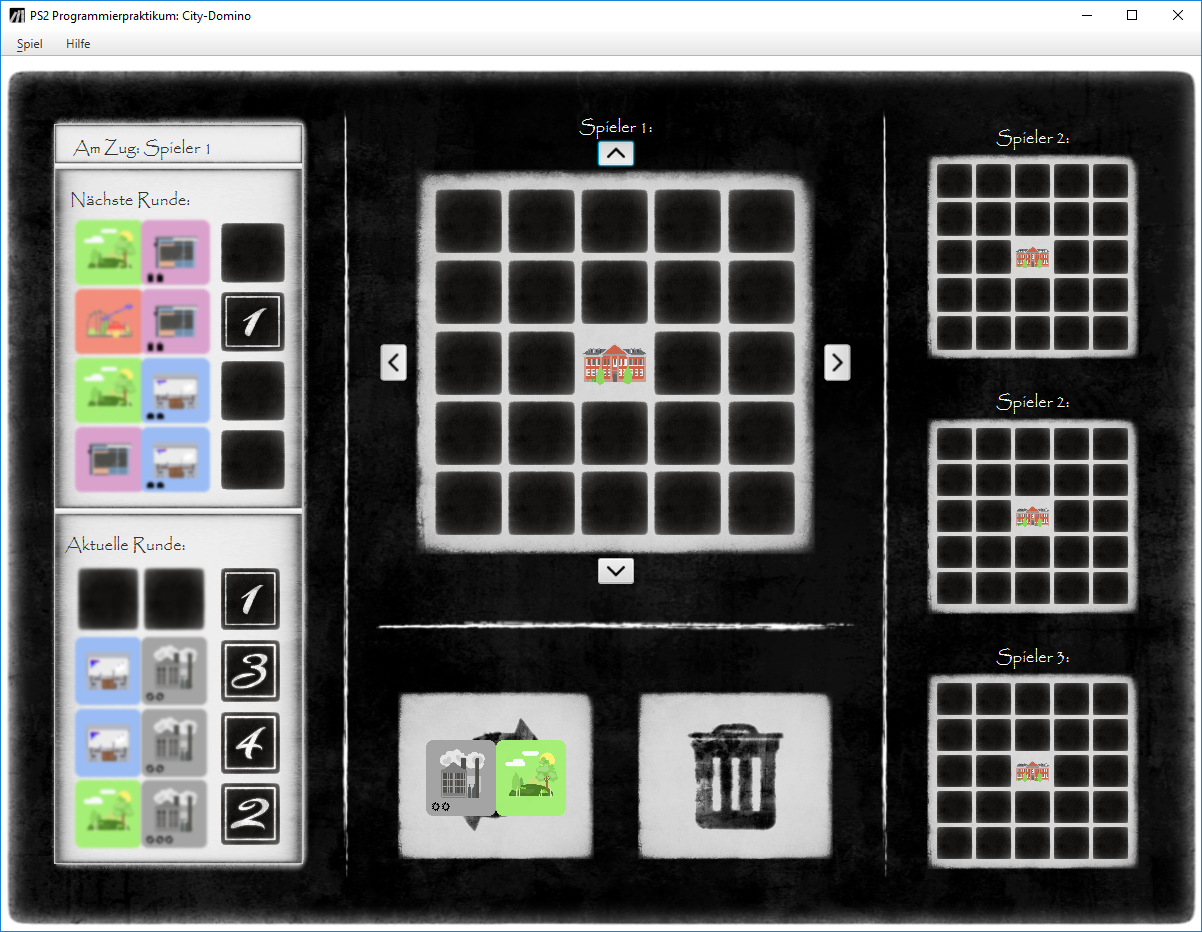
\includegraphics{screenshots/screenshot_ErstesSelektierenAufNaechsterBank}
	\caption[Erstes Selektieren]{Erstes Selektieren auf der Bank fuer die naechste Runde}
	\label{fig:erstesSelektierenNaechsteBank}
\end{figure}

\subparagraph{Justierung des Dominos}
Nachdem der Spieler erfolgreich saemtliche Selektierungsschritte auf den beiden Baenken absolviert hat, kann er seinen zuvor ausgewaehlten Domino in dem dafuer vorgesehenen Kasten drehen. Um den Domino um 90 Grad zu drehen muss der Spieler lediglich einen Mausklick auf dem Domino ausfuehren. 

\subparagraph{Positionierung auf dem Spielfeld}
Um den justierten Domino nun auf dem Feld zu platzieren zieht der Benutzer den Domino an die gewuenschte Stelle auf dem Spielfeld. Waehrend dem Ziehen faerben sich zugrunde liegenden Felder jeweils gruen, falls es moeglich sein sollte den Domino an dieser Stelle anzulegen (siehe Abbildung \pageref{fig:hovernGruen}), beziehungsweise rot, falls dies nicht der Fall sein sollte (siehe Abbildung \ref{fig:hovernRot}, fuer genauere Informationen siehe Abschnitt \ref{par:anlegeregeln}). Falls der Domino an der gewuenschten Stelle nicht passen sollte und dennoch versucht wird ihn an dieser Stelle zu platzieren, passiert nichts denn der Domino befindet sich weiterhin in dem Kasten zum justieren der Ausrichtung und es kann ein neuer Versuch gestartet werden. 

\subparagraph{Verwerfen des Dominos}
Um den Domino zu verwerfen reicht es per Mausklick einmal auf das Muelleimer-Symbol rechts neben dem Domino zu klicken. Der Domino wird anschliessend aus dem Rotationsfeld entfernt. 

\begin{figure}
	\centering
	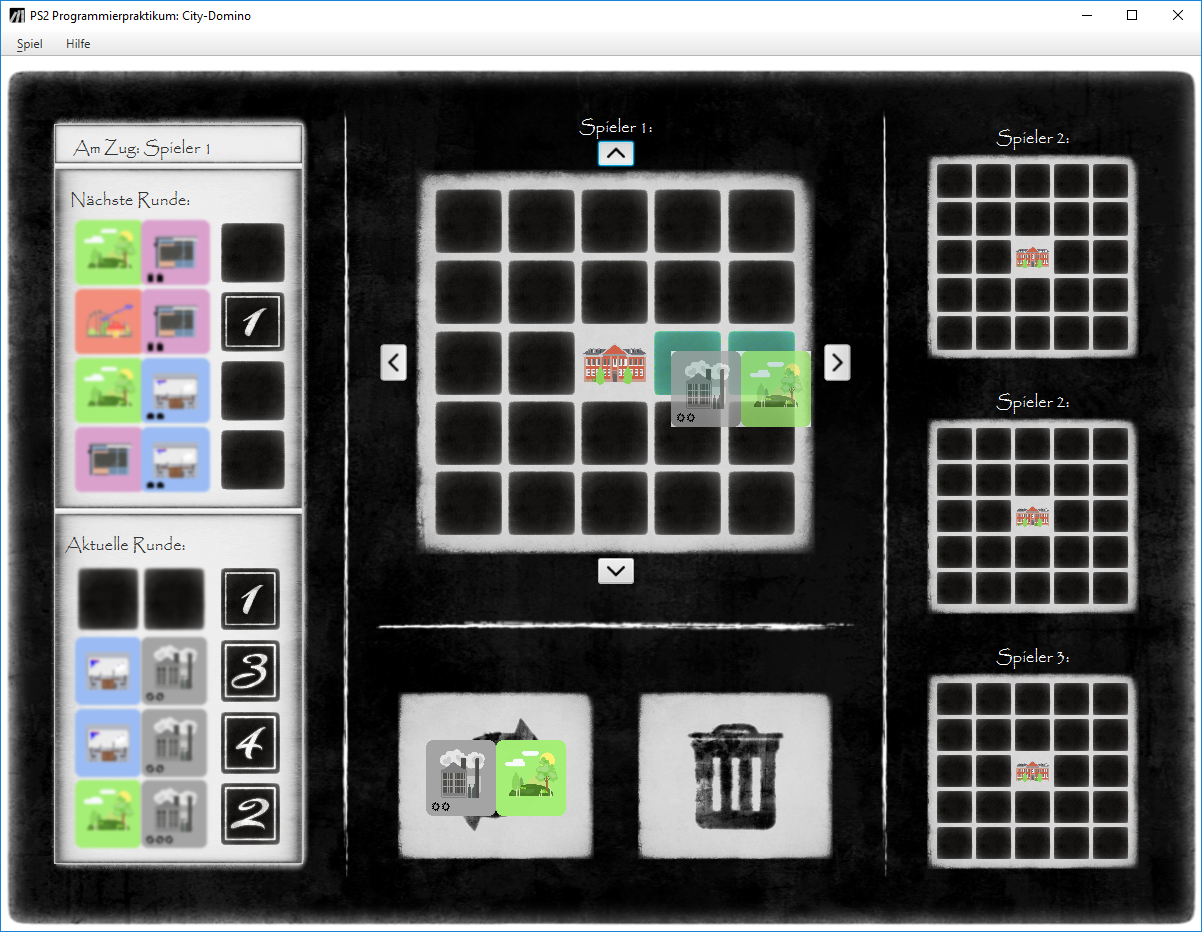
\includegraphics{screenshots/screenshot_HovernGruen}
	\caption{Schwebender Domino ueber gueltiger Position}
	\label{fig:hovernGruen}
\end{figure}

\begin{figure}
	\centering
	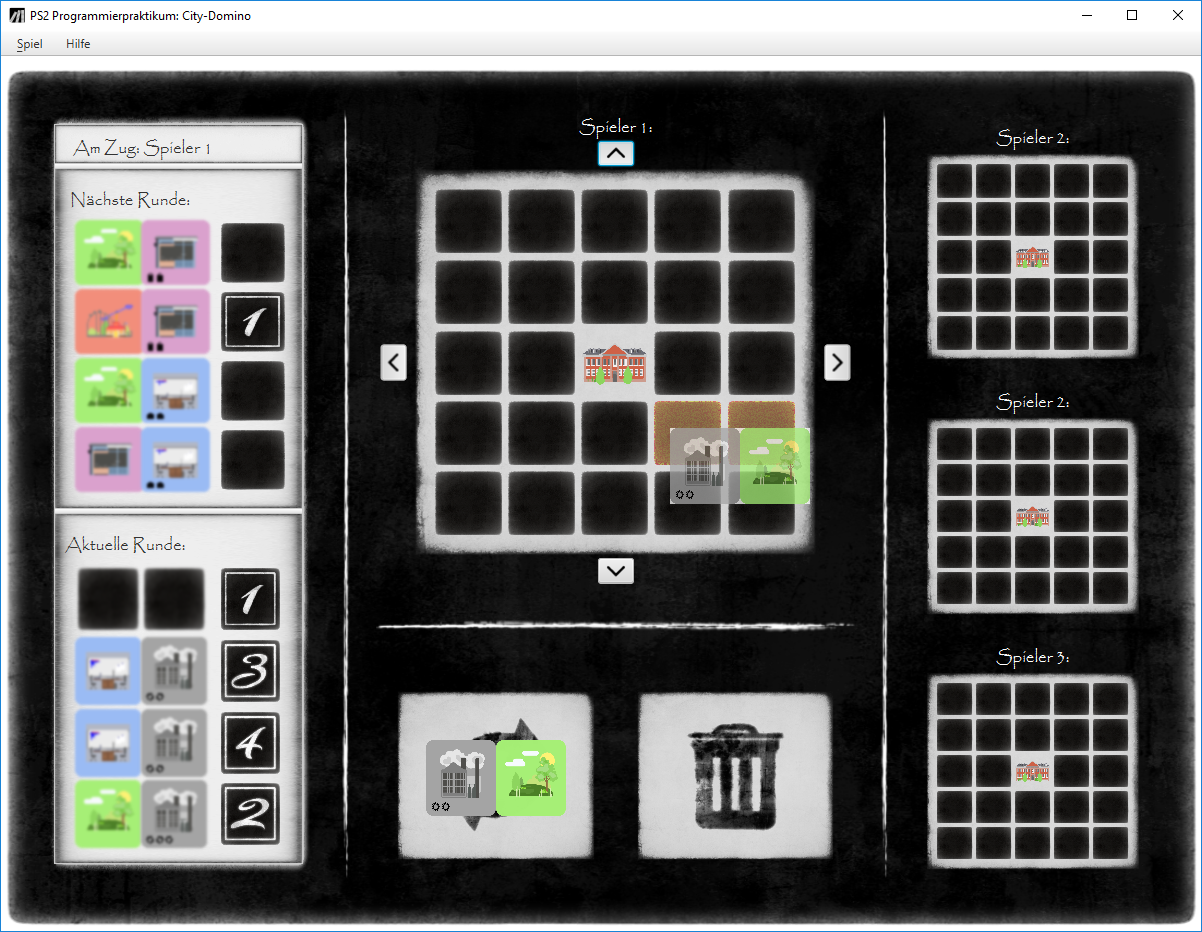
\includegraphics{screenshots/screenshot_HovernRot}
	\caption{Schwebender Domino ueber ungueltiger Position}
	\label{fig:hovernRot}
\end{figure}


\newpage

\begin{figure}
	\centering
	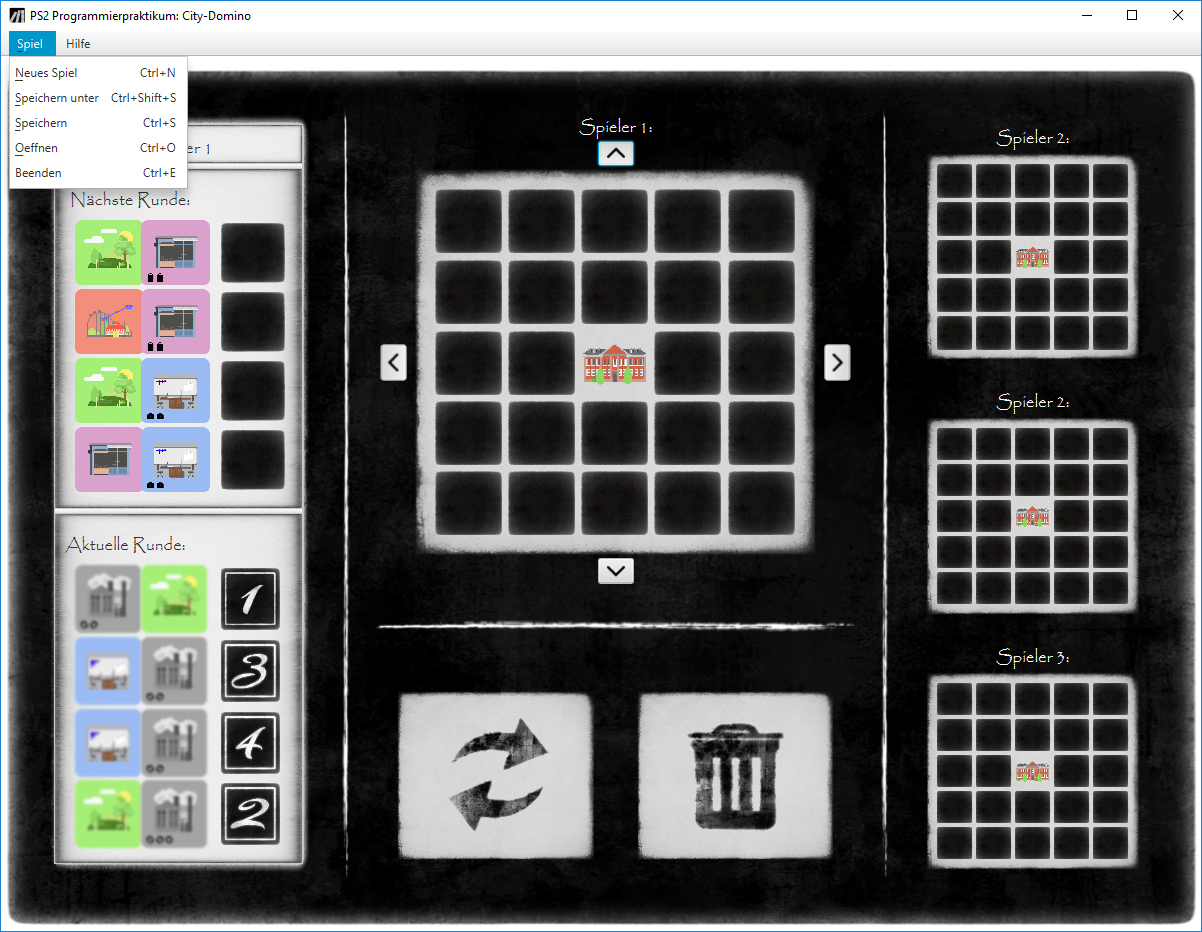
\includegraphics{screenshots/screenshot_Menue}
	\caption{Menueoptionen}
	\label{fig:menueoptionen}
\end{figure}

\paragraph{Menueinteraktion}
\subparagraph{Starten bzw. Schliessen}
Um ein neues Spiel zu starten waehlt der Benutzer den Menuepunkt "\emph{Neues Spiel}". Alternativ ist dies auch per Tastenkombination \verb|strg + N| moeglich. Um das geoffnete Fenster zu schliessen und das bestehende Spiel zu verwerfen waehlt der Benutzer den Reiter \emph{Beenden} (Tastenkombination \verb|strg + E|). Falls der Benutzer das Spiel nicht vorher gespeichert hat erscheint hierbei ein weiteres Fenster welches den Benutzer darauf hinweist und ihm die Moeglichkeit gibt dies nachzuholen (siehe folgenden Abschnitt). Moechte er fortfahren ohne den aktuellen Spielstand muss der Button mit der Aufschrift \emph{Abbrechen} betaetigt werden (siehe Abbildung \ref{fig:nachtrSpeichern}). 

\begin{figure}
	\centering
	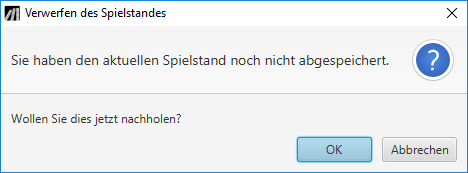
\includegraphics[width=.6\linewidth]{screenshots/screenshot_NachtraeglichesAbspeichern}
	\caption{Nachtraegliches Abspeichern}
	\label{fig:nachtrSpeichern}
\end{figure}

\subparagraph{Spielstand abspeichern}
\label{spar:anleitung_speichern}
Um ein Spielstand zu speichern gibt es zwei Reiter mit folgenden Moeglichkeiten.
\begin{enumerate}
	\item{Speichern: \verb|Strg + S|}
	\item{Speichern unter: \verb|Strg + Shift + S|}
\end{enumerate}
Speichern unter gibt dem Benutzer die Moeglichkeit, ausgehend vom Ablageverzeichnis den gewuenschten Speicherort anzugeben. Hierzu navigiert man mit dem gegebenen Filechooser an den gewuenschten Speicherort und gibt der abzuspeichernden Datei einen Namen, die benoetigt Dateiendung \emph{.txt} ist bereits ausgewaehlt, sodass der Benutzer seine Auswahl lediglich auf dem Feld \emph{Speichern} per Mausklick zu bestaetigen braucht (siehe Abbildung \ref{fig:filechooser}). 

Der Reiter \emph{Speichern} ermoeglicht es einen bereits gespeicherten Spielstand ohne oeffnen eines Filechoosers zu ueberschreiben. Falls der Benutzer diesen Reiter betaetigt ohne dass zuvor ein Spielstand des aktuellen Spiels abgespeichert wurde ist, oeffnet sich bei der Auswahl dieses Reiters dennoch ein Filechooser und es wird nach der Funktionsweise von \emph{Speichern unter} vorgegangen. 

\subparagraph{Oeffnen}
Aehnlich wie beim Reiter \emph{Speichern unter} wird hier ein Filechooser geoeffnet. Dieser wird jedoch dazu verwendet eine Datei auszuwaehlen um aus dieser einen Spielstand zu lesen. Falls die Datei nicht der geforderten Syntax entspricht, erscheint eine Fehlermeldung in Form eines Popup-Fensters mit dem einer groben Fehlermeldung wo der Fehler liegt \lstref{fig:Fehleruebersicht}. Falls der Benutzer vor dem Oeffnen eines neuen Spielstands den alten nicht gespeichert hat wird er aehnlich wie beim Beenden darauf hingewiesen und es wird per Filechooser eine Moeglichkeit bereitgestellt dies nachzuholen.

\begin{figure}
	\centering
	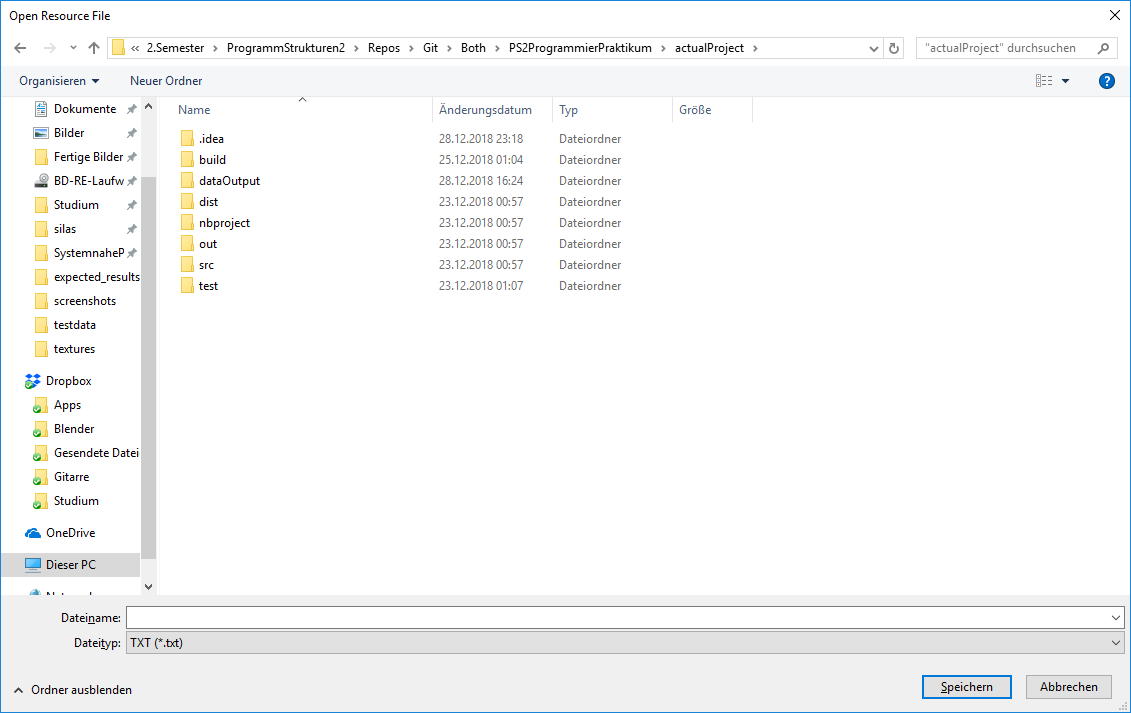
\includegraphics{screenshots/screenshot_Filechooser}
	\caption[Filechooser]{Filechooser zum Abspeichern eines Spielstandes}
	\label{fig:filechooser}
\end{figure}

\begin{figure*}
        \centering
        \begin{subfigure}[b]{0.35\textwidth}   
            \centering 
            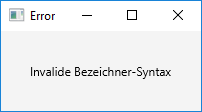
\includegraphics[width=\textwidth]{screenshots/screenshot_ErrorBezeichner}
            \caption[]%
            {{\small Bezeichner}}    
            \label{fig:BezeichnerErr}
        \end{subfigure}
        \quad
        \begin{subfigure}[b]{0.35\textwidth}   
            \centering 
            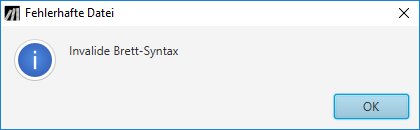
\includegraphics[width=\textwidth]{screenshots/screenshot_ErrorBrett}
            \caption[]%
            {{\small Brett}}    
            \label{fig:BrettErr}
        \end{subfigure}
        \vskip\baselineskip
        \begin{subfigure}[b]{0.35\textwidth}   
            \centering 
            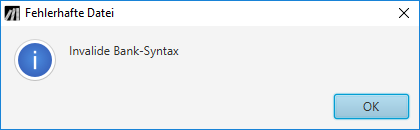
\includegraphics[width=\textwidth]{screenshots/screenshot_ErrorBank}
            \caption[]%
            {{\small Bank}}    
            \label{fig:BankErr}
        \end{subfigure}
        \quad
        \begin{subfigure}[b]{0.35\textwidth}   
            \centering 
            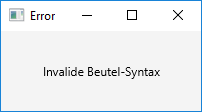
\includegraphics[width=\textwidth]{screenshots/screenshot_ErrorBeutel}
            \caption[]%
            {{\small Beutel}}    
            \label{fig:BeutelErr}
        \end{subfigure}
        \caption
        {\small Unterschiedliche Fehlermeldungen beim Einlesen einer Datei} 
        \label{fig:Fehleruebersicht}
    \end{figure*}

\subparagraph{Hilfestellung}
Unter dem Reiter \emph{Hilfe} ist die Aufgabenstellung im Pdf-Format zu finden. Beim Auswaehlen des Menuepunktes \emph{Aufgabenstellung} oeffnet sich diese im, vom Benutzer standardmaessig genutzten, Pdf-Reader. 


\subsection{Programmfunktionalitaet}
Generell gilt es zwischen einem standardmaessig ausgefuehrten Spiel und einem eingelesenem Spiel zu unterscheiden. 

\paragraph{Spiel ohne Einlesen einer Datei}
\subparagraph{Spielbeginn}
\emph{Ein Spielbeutel für alle Spieler enthält 48 Spielkarten in der Größe von zwei Zellen, die auf ihren zwei Hälften jeweils einen (evtl. auch den gleichen) Stadtteiltyp anzeigen. Die Stadtteiltypen unterscheiden sich durch Bild und Hintergrundfarbe voneinander. Jede Spielkarte besitzt eine definierte Wertigkeit. Auf manchen Stadtteilen sind zusätzlich ein bis drei Prestigesymbole abgebildet. Jeder Spieler besitzt ein eigenes 5*5-Zellen großes Spielfeld und legt zu Beginn sein Stadtzentrum mittig ab}
\cite{aufgabenstellung}. 
(siehe Abbildung \ref{fig:spielbeginnGui}). Dies wird bereits vom Spiel uebernommen, sodass der erste Spielzug des Benutzers das initiales Selektieren vom ersten Auswahlbereich (hier mit \emph{Aktuelle Runde} gekennzeichnet) darstellt. Um einen Domino selektieren zu koennen \emph{ werden vier Karten gezogen und im ersten Auswahlbereich angezeigt. Dabei wird die niederwertigste Karte zuoberst, die höchstwertigste zuunterst einsortiert. Der erste Spieler markiert die Karte im Auswahlbereich, die er gerne nehmen würde, die anderen Spieler treffen ihre Auswahl der Reihe nach ebenfalls und markieren die jeweils gewünschte Karte. Wurden alle Karten markiert, dann werden wieder vier Karten gezogen und ebenso sortiert im zweiten Auswahlbereich angezeigt.} 
\cite{aufgabenstellung}
(Siehe Abbildung \ref{fig:initialesSelektierenOben})

\begin{figure}
	\centering
	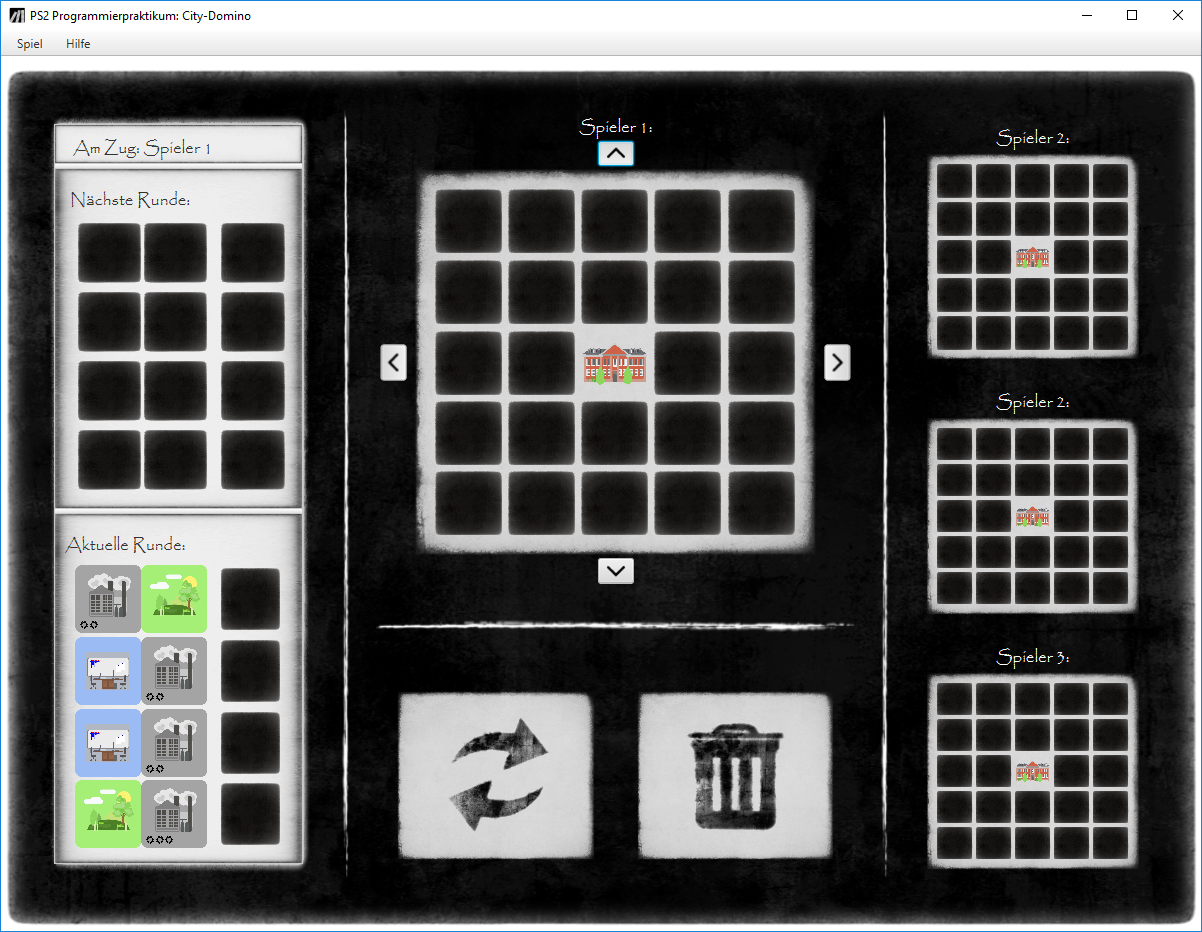
\includegraphics{screenshots/screenshot_Spielbeginn.png}
	\caption[Spielbeginn]{Spielbeginn nach Programmstart}
	\label{fig:spielbeginnGui}
\end{figure}


\begin{figure}
	\centering
	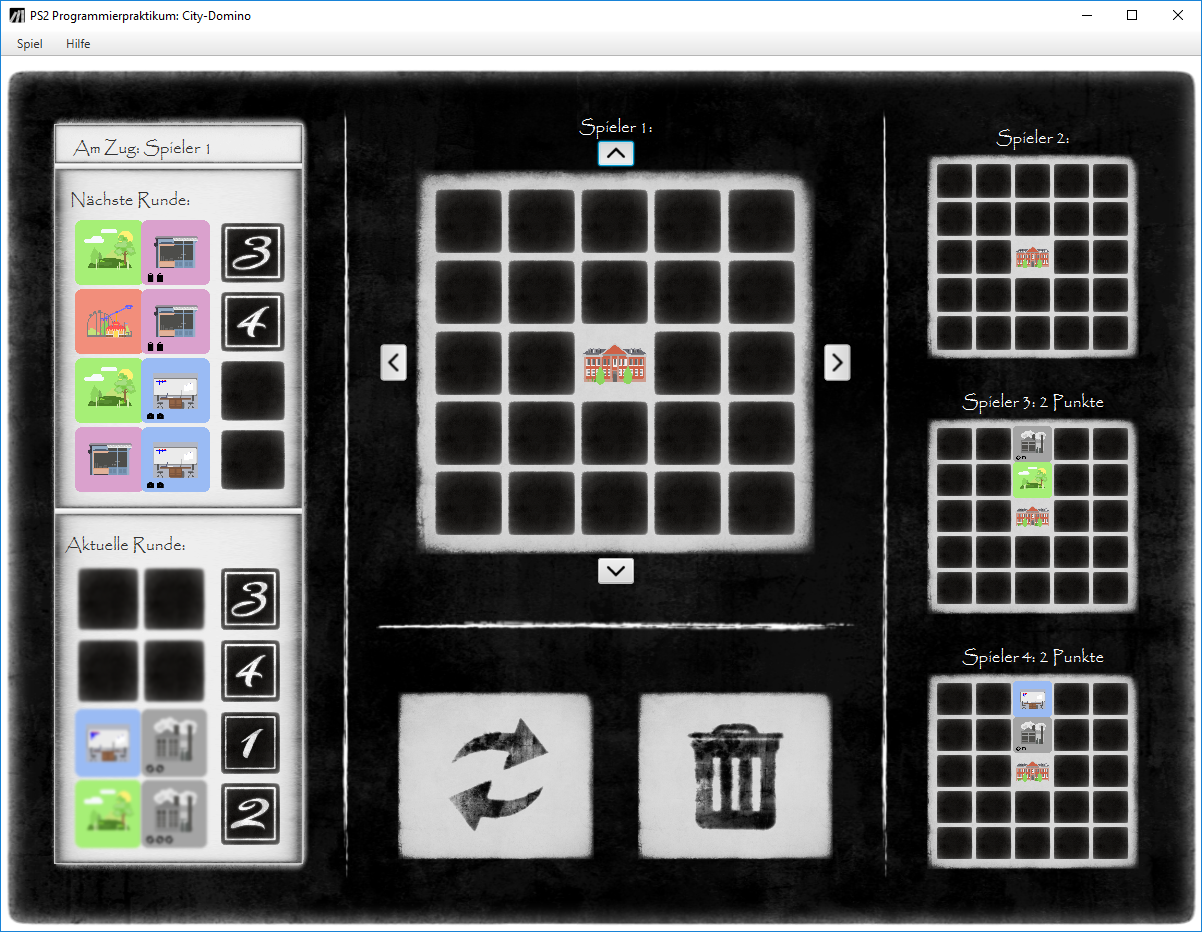
\includegraphics{screenshots/screenshot_InitialesSelektieren2.png}
	\caption[Initiales Selektieren - oben]{Initiales Selektieren (oben) nach Programmstart}
	\label{fig:initialesSelektierenOben}
\end{figure}

\subparagraph{Spielablauf}
\emph{Derjenige, der die oberste Karte im ersten Auswahlbereich markiert hat, beginnt eine Runde, es folgen der Reihe
nach die Spieler, die die jeweils darunterliegende Karte markiert haben. In einer Runde wird zunächst eine Karte
aus dem zweiten Auswahlbereich markiert und dadurch für die kommende Runde gewählt. Je wertvoller also seine
markierte Karte in dieser Runde ist, desto später ist der Spieler am Zug und desto weniger Auswahl hat er für die
kommende Runde.}
\cite{aufgabenstellung}
Zwischen dem initialen Selektieren und dem beschriebenen Spielablauf gibt es keine Pause. Wie man in Abbildung \ref{fig:initialesSelektierenMittig} sehen kann, ziehen die Gegner bereits ihre ersten Dominos auf ihr Feld wo der Benutzer noch gar nicht an der Reihe war. Nun kann der Benutzer einen Domino auf dem naechsten Auswahlstapel bzw. der naechsten Bank einen der uebrig gebliebenen Dominosteine auswaehlen. Nun wird der Domino welcher als erstes Selektiert wurde in den Kasten zum rotieren geladen (siehe Abbildung \ref{fig:erstesRotieren}) und der Benutzer kann den Stein auf sein Brett legen (Abbildung \ref{fig:ersteAblage}). Nach dieser Aktion kann der Benutzer einen Domino auf der Bank fuer die naechste Runde auswaehlen. Danach muss er wieder "warten" bis er an der Reihe ist um einen ausgewaehlten Domino auf seinem Brett zu platzieren. Alternativ kann er seinen Domino aber auch verwerfen.

\begin{figure}
	\centering
	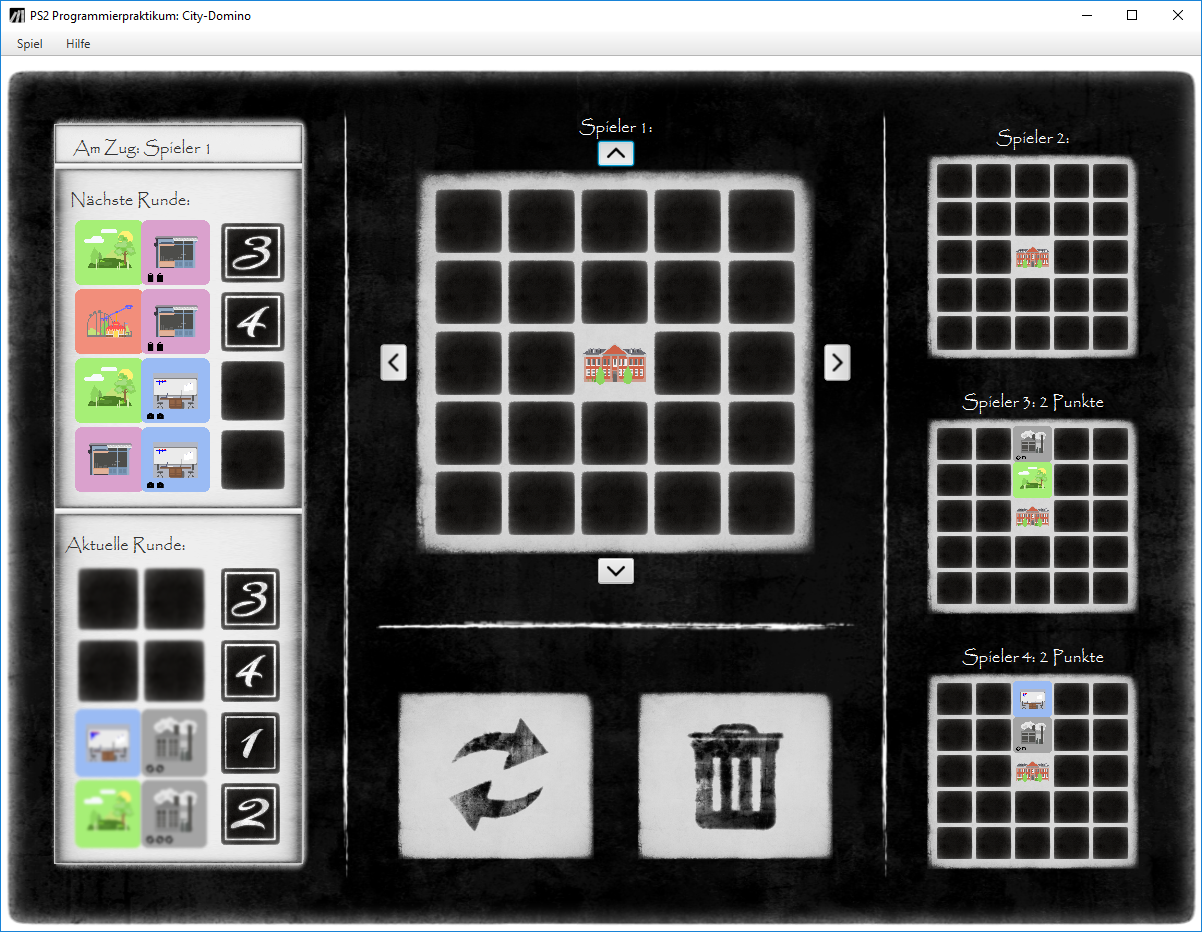
\includegraphics{screenshots/screenshot_InitialesSelektieren2.png}
	\caption[Initiales Selektieren - mittig]{Initiales Selektieren (mittig) nach Programmstart}
	\label{fig:initialesSelektierenMittig}
\end{figure}


\begin{figure}
	\centering
	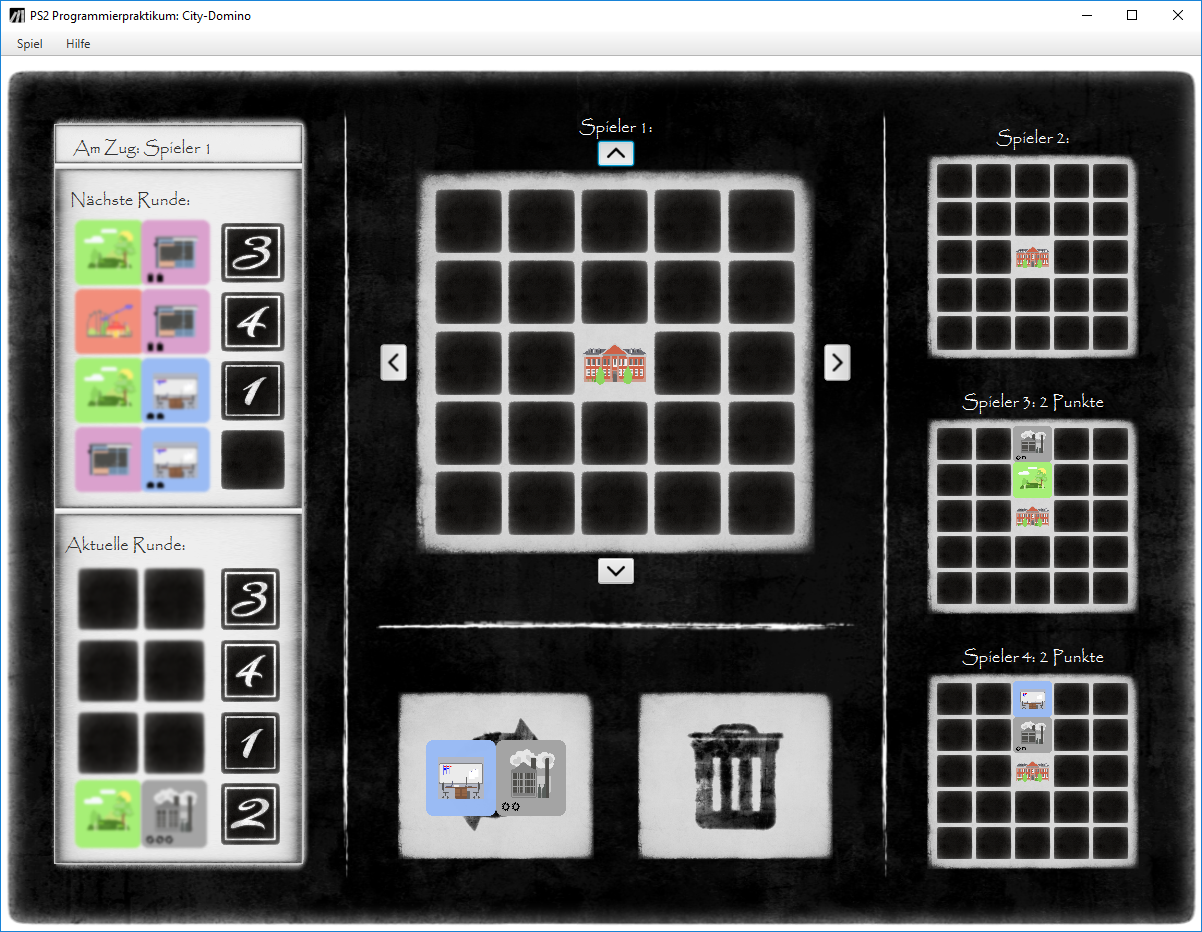
\includegraphics{screenshots/screenshot_ErstesRotieren.png}
	\caption{Erstes Rotieren}
	\label{fig:erstesRotieren}
\end{figure}

\begin{figure}
	\centering
	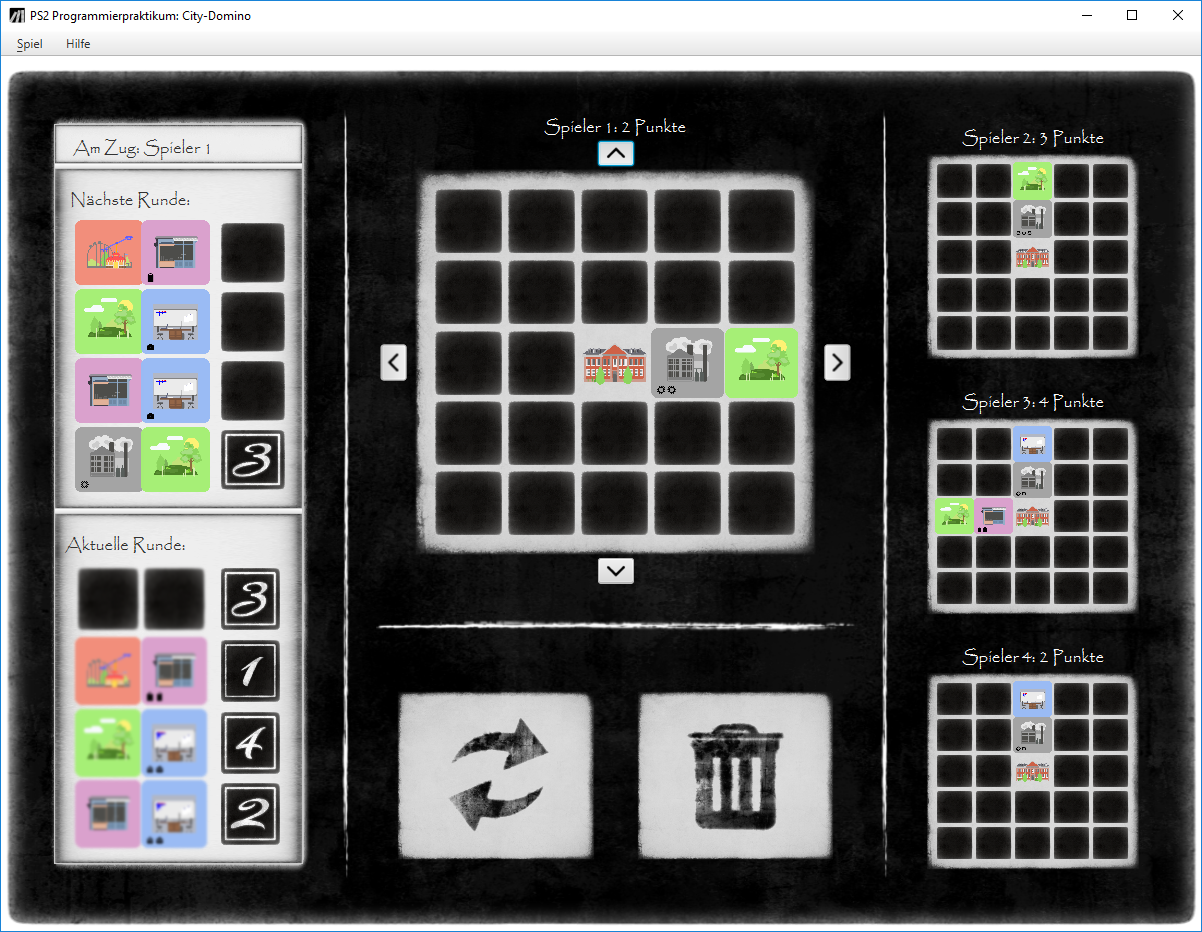
\includegraphics{screenshots/screenshot_ErsteAblage.png}
	\caption[Erste Ablage]{Erste Ablage auf dem Spielfeld}
	\label{fig:ersteAblage}
\end{figure}

\paragraph{Einlesen einer Datei}
Nachdem der Benutzer eine Datei eingelesen hat ist dieser auch gleichzeitig am Zug. Je nachdem ob der Spielstand waehrend des initialen Selektierens oder waehrend einer standardmaessigen Runde abgespeichert wurde, muss der Benutzer entweder von der Bank fuer die aktuelle Runde oder von der Bank der naechsten Runde Selektieren. Generell gelten hier die gleichen Regeln zum Spielablauf wie beim Spielen ohne gespeicherten Spielstand, es kann nur der Schritt des initialen Selektierens uebersprungen werden. 

\paragraph{Anlegeregeln}
\emph{Die erste Karte muss an das Stadtzentrum angrenzen. An das Stadtzentrum darf jeder Stadtteil angrenzen. Legt man eine Karte an eine andere Karte an, so muss mindestens eine Hälfte mit einer Seite an einen identischen Stadtteiltyp einer liegenden Karte angrenzen. Passt die abzulegende Karte weder an das Stadtzentrum noch an eine bereits ausliegende Karte, so wird sie verworfen. Alle Spielkarten müssen in das 5*5-Feld passen, keine Hälfte darf hinausragen. Das Stadtzentrum muss aber nicht in der Mitte liegen, sondern kann im Spielverlauf verschoben werden, wodurch sich alle bereits gelegten Karten mit verschieben. Eine abgelegte Karte kann nicht verschoben werden.}
\cite{aufgabenstellung}

\paragraph{Spielende}
\emph{Wurden alle Spielkarten aus dem Beutel gezogen und von den
Auswahlbereichen auf die Spielfelder platziert bzw. verworfen, werden die
Punkte ermittelt.
\begin{itemize}
	\item Jede Stadt besteht aus mehreren Stadtteilen. Ein Stadtteil setzt sich aus waagerecht und/oder senkrecht verbundenen Zellen desselben Stadtteiltyps zusammen. Das Stadtzentrum zählt zu keinem Stadtteil dazu
	\item Die Punkte eines Stadtteils ergeben sich aus der Anzahl seiner Zellen
multipliziert mit der Anzahl darin enthaltener Prestigesymbole.
	\item Innerhalb einer Stadt kann es mehrere voneinander getrennte Stadtteile
desselben Typs geben. Jeder Stadtteil ist einzeln auszuwerten. Stadtteile ohne Prestigesymbole bringen keine Punkte. 
\end{itemize}
Für die Auswertung wird für jeden Spieler die Summe der Punkte seiner Gebiete ermittelt. Gewonnen hat der Spieler mit den meisten Punkten. Bei einem Gleichstand gewinnt der Spieler mit dem größten einzelnen Gebiet. Besteht auch hier Gleichstand, so siegen beide Spieler gleichermaßen.
}
\cite{aufgabenstellung}



\label{par:anlegeregeln}